\chapter{P, L, R and the dual graph}\label{ch:plr}

\section{Three parsimonious operations}
Two triangles of the Tonnetz share an edge exactly when the two triads share two notes. For each triad there are
three such neighbours, one across each edge, and they define three involutions on the set of 24 triads:
\begin{description}[leftmargin=1.2em]
\item[$P$ (parallel)] keeps the root and fifth and moves the third by a semitone: C $\leftrightarrow$ Cm.
\item[$L$ (leading-tone exchange)] keeps the third and fifth of a major triad and lowers the root a semitone:
C $\leftrightarrow$ Em (C--E--G $\to$ B--E--G).
\item[$R$ (relative)] keeps the root and third of a major triad and raises the fifth a whole tone:
C $\leftrightarrow$ Am (C--E--G $\to$ C--E--A).
\end{description}
In the lattice picture (\cref{fig:lattice}), $P$ flips a triangle across its fifth-edge, $L$ across its
minor-third edge and $R$ across its major-third edge. Each is its own inverse ($P^2=L^2=R^2=\mathrm{id}$) and each
swaps major and minor. Measured as total semitone motion of the voices, $P$ and $L$ cost 1 and $R$ costs 2; these
are the smallest possible voice leadings between a major and a minor triad, which is what Cohn means by
\emph{parsimonious} \citep{cohn1997}.

\section{The dual graph}
\begin{definition}
The \emph{$PLR$ graph} $\Gamma$ has the 24 consonant triads as vertices and an edge labelled $P$, $L$ or $R$ between
$t$ and $P(t)$, $L(t)$, $R(t)$.
\end{definition}
$\Gamma$ is the dual of the triangulated Tonnetz: vertices of $\Gamma$ are triangles of the Tonnetz and edges of $\Gamma$
cross edges of the Tonnetz. Drawn in the plane it is a hexagonal honeycomb (\cref{fig:dual}), and on the torus it
is Douthett and Steinbach's ``chicken-wire torus'' \citep{douthett1998}.

\begin{figure}[t]\centering
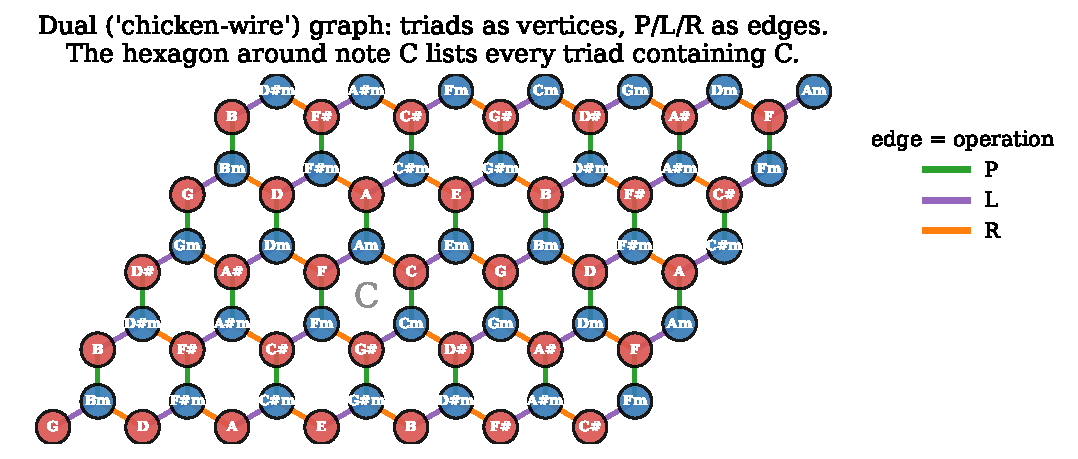
\includegraphics[width=0.9\linewidth]{figures/dual_graph.pdf}
\caption{A patch of the dual graph. Red vertices are major and blue are minor triads; edge colour gives the
operation. Every hexagonal face corresponds to one note of the Tonnetz and lists the six triads containing it.}
\label{fig:dual}
\end{figure}

\begin{proposition}\label{prop:gamma}
$\Gamma$ is connected, cubic, bipartite (majors versus minors) and has 24 vertices, 36 edges and diameter 5.
From any triad, the numbers of triads at distance $1,2,3,4,5$ are $3,6,8,5,1$.
\end{proposition}
\begin{proof}[Proof sketch]
Cubic and bipartite follow from the definitions ($P,L,R$ are distinct and each changes the mode). Edges:
$24\cdot3/2=36$. The distance profile is the same from every vertex because $D_{12}$ acts transitively and
commutes with $P,L,R$ (below); it is checked by breadth-first search in \sheet{03\_plr\_dual.ipynb}. The unique
triad at distance 5 from C major is B$\flat$ minor.
\end{proof}

\section{Faces and famous cycles}
Three families of short cycles in $\Gamma$ are central to neo-Riemannian analysis.

\paragraph{Hexagons: the triads around a note.} Alternately applying $P$, $L$, $R$ six times returns to the start.
From C, $(PLR)^2$ visits C, Cm, A$\flat$, Fm, F, Am: precisely the six triads that contain the note C. These
hexagons are the faces of $\Gamma$ on the torus; there are 12 of them, one per pitch class, and $\Gamma$ has
$V-E+F=24-36+12=0$, as a graph embedded in the torus must.

\paragraph{Hexatonic cycles.} $(PL)^3$ from C gives C, Cm, A$\flat$, A$\flat$m, E, Em: the six triads contained in
the hexatonic scale $\{0,3,4,7,8,11\}$. There are four such cycles, Cohn's \emph{hexatonic systems}
\citep{cohn1996}, central to his account of late-Romantic ``maximally smooth'' progressions.

\paragraph{Octatonic cycles.} $(PR)^4$ gives eight triads (C, Cm, E$\flat$, E$\flat$m, F$\sharp$, F$\sharp$m, A, Am) in an
octatonic scale; there are three such cycles.

\paragraph{The $LR$ chain.} $(LR)^{12}$ visits all 24 triads, alternating major and minor while the major roots
descend (or ascend) by fifths: C, Em, G, Bm, D, $\dots$ Long stretches of this chain occur in the repertoire; a
celebrated example is a passage in the scherzo of Beethoven's Ninth Symphony discussed by Cohn \citep{cohn1997}.
We meet this cycle again as the most symmetric Hamiltonian cycle in Chapter~\ref{ch:ham}.

\begin{correctionbox}
The slide ``Hamiltonian cycles (again)'' states that ``going around a hexagon'' gives
C $\to$ Am $\to$ F $\to$ Dm $\to$ G $\to$ Em $\to$ C. Checking each step against $\Gamma$ shows that five steps are
edges ($R,L,R$ and then $R,L$) but Dm $\to$ G is not: D--F--A and G--B--D share only one note (PLR distance 3).
The progression is a diatonic chain of falling thirds, not a face of the dual graph. The hexagon through C and Am
is C--Cm--A$\flat$--Fm--F--Am (the triads containing C), or, around the note E, C--Em--E--C$\sharp$m--A--Am.
\end{correctionbox}

\section{The $PLR$ group and its dual}
Let $\mathcal{G}=\langle P,L,R\rangle$ be the group of permutations of the 24 triads generated by the three
involutions. A direct computation (\sheet{03\_plr\_dual.ipynb}) shows $|\mathcal G|=24$; in fact $\mathcal G$ is
already generated by $L$ and $R$, since $RL$ has order 12, and $\mathcal G\cong D_{12}$. The deeper structural
fact is:

\begin{theorem}[Crans--Fiore--Satyendra \citep{crans2009}]
The $PLR$ group and the $T/I$ group are both dihedral of order 24, each acts simply transitively on the
consonant triads, and each is the centraliser of the other in the symmetric group on the 24 triads.
\end{theorem}
Informally: $P$, $L$ and $R$ are defined by \emph{internal} features of a chord (``keep root and fifth'') rather
than by absolute pitch, so they commute with transposition and inversion. For example
$P(T_5\,t)=T_5\,P(t)$ for every triad $t$; the notebook verifies this for all 24 triads. Transformational theorists
call this relationship \emph{duality} (Lewin's ``simply transitive group action'' \citep{lewin1987}); it explains
why a neo-Riemannian analysis can be transposed freely.

\section{Two metrics on triads}
Distances in $\Gamma$ count single-voice moves; the \emph{voice-leading distance} instead minimises the total
number of semitones moved, over all ways of pairing the notes. They agree on edges only up to the factor that
$R$ costs 2, and diverge more for larger moves: C $\to$ G (a fifth up) is two steps in $\Gamma$ ($L$ then $R$) with
voice-leading cost 3, while F $\to$ G (a whole step, as in IV $\to$ V) is four steps in $\Gamma$ with voice-leading
cost 6. This difference matters for the corpus study of Chapter~\ref{ch:data}.

\begin{notebookbox}
\sheet{03\_plr\_dual.ipynb}: build $\Gamma$, verify \cref{prop:gamma}, list the hexagonal, hexatonic and octatonic
cycles, test the slide's progression edge by edge, and generate $\langle P,L,R\rangle$.
\end{notebookbox}

\begin{qa}
\Qu{Compute $P$, $L$ and $R$ of A minor.}
\A{$P(\text{Am})=\text{A}$ (C$\to$C$\sharp$), $L(\text{Am})=\text{F}$ (E$\to$F), $R(\text{Am})=\text{C}$
(A$\to$G).}
\Qu{Why is $\Gamma$ bipartite?}
\A{Each of $P$, $L$, $R$ changes the mode, so every edge joins a major triad to a minor triad.}
\Qu{How many hexagonal faces does $\Gamma$ have on the torus, and why?}
\A{Twelve: each face is the set of triads containing a fixed note, and there are 12 notes. Check:
$\chi=24-36+12=0$.}
\Qu{Which triads lie on the hexatonic cycle through D major?}
\A{$(PL)^3$ from D: D, Dm, B$\flat$, B$\flat$m, F$\sharp$, F$\sharp$m.}
\Qu{Why do $P,L,R$ commute with transposition?}
\A{They are defined relative to a chord's own root, third and fifth, and transposition moves all three together;
so transposing first and then applying $P$ gives the same result as applying $P$ then transposing.}
\Qu{Give a progression that is short in voice-leading terms but long in $\Gamma$.}
\A{F $\to$ G: every voice moves a whole step (cost 6, small as a gesture and idiomatic as IV--V) but it takes four
$P/L/R$ steps, e.g.\ F$\xrightarrow{R}$Dm$\xrightarrow{L}$B$\flat\xrightarrow{R}$Gm$\xrightarrow{P}$G.}
\end{qa}
